\documentclass{beamer}
% Copyright 2015 by Do Phan Thuan

% Loại mẫu slice
%\usetheme{AnnArbor}
%\usetheme{Antibes}
\usetheme{Boadilla}
%\usetheme{CambridgeUS}
%\usetheme{Hannover}

% Ký tự tiếng Việt
\usepackage[utf8]{vietnam}
\usepackage[utf8]{inputenc}
% Công thức toán
\usepackage{amsmath,amsthm,amssymb,epsfig}
% Chèn ảnh
\usepackage{graphicx}
% Chèn đường dẫn 
\usepackage{url}

% Vẽ đồ thị
\usepackage{pgfplots}

% Insert code
\usepackage{listings}
\lstset{language=C++,
   %keywords={break,case,catch,continue,else,elseif,end,for,function,
   %   global,if,otherwise,persistent,return,switch,try,while},
   basicstyle=\ttfamily,
   keywordstyle=\color{blue},
   commentstyle=\color{red},
   stringstyle=\color{dkgreen},
   frame=lrtb,
   %frame=5 pt,
   numbers=left,
   numberstyle=\tiny\color{gray},
   stepnumber=1,
   numbersep=10pt,
   backgroundcolor=\color{white},
   tabsize=4,
   showspaces=false,
   showstringspaces=false}
% Tô mầu cho bảng
\usepackage{colortbl}


\usepackage{color}

\definecolor{dkgreen}{rgb}{0,0.6,0}
\definecolor{gray}{rgb}{0.5,0.5,0.5}
\definecolor{mauve}{rgb}{0.58,0,0.82}
  
\definecolor{Xanh}{rgb}{0,0.5,1}
\definecolor{Do}{rgb}{1,0.25,0}
\definecolor{Vang}{rgb}{1,1,0}
\definecolor{Datroi}{rgb}{0,0,1}
% Vẽ hình
\usepackage{tikz}
\usetikzlibrary{arrows,shapes}
% Vẽ mạch điện
\usepackage[siunitx,european resistors]{circuitikz}

% multirow
\usepackage{multirow}

\usepackage{pbox}

% Tô mầu cho bảng
\usepackage{colortbl}
\definecolor{Xanh}{rgb}{0,0.5,1}
\definecolor{Do}{rgb}{1,0.25,0}
\definecolor{Vang}{rgb}{1,1,0}
\definecolor{Datroi}{rgb}{0,0,1}

% Một vài ký hiệu thường dùng
\def\R{{\mathbb R}}
\def\N{{\mathbb N}}
\def\X{{\mathcal X}}
\def\Y{{\mathcal Y}}
\def\F{{\mathcal F}}
\def\P{{\mathcal P}}
\def\E{{\mathbb E}}
\def\I{{\mathbb I}}
\def\sign{{\rm sign}}

% Xác định khoảng dãn trong bảng
\renewcommand\arraystretch{1.2}

% a few macros
\newcommand{\bi}{\begin{itemize}}
\newcommand{\ei}{\end{itemize}}
\newcommand{\ig}{\includegraphics}
\newcommand{\subt}[1]{{\footnotesize \color{subtitle} {#1}}}

% named colors
\definecolor{offwhite}{RGB}{249,242,215}
\definecolor{foreground}{RGB}{255,255,255}
\definecolor{background}{RGB}{24,24,24}
\definecolor{title}{RGB}{107,174,214}
\definecolor{gray}{RGB}{155,155,155}
\definecolor{subtitle}{RGB}{102,255,204}
\definecolor{hilight}{RGB}{22,155,104}
\definecolor{vhilight}{RGB}{255,111,207}
\definecolor{lolight}{RGB}{155,155,155}
%\definecolor{green}{RGB}{125,250,125}

% Minted
%\usepackage{minted}
%\usemintedstyle{monokai}
%\newminted{cpp}{fontsize=\footnotesize}

% Graph styles
\tikzstyle{vertex}=[circle,fill=black!50,minimum size=15pt,inner sep=0pt, font=\small]
\tikzstyle{selected vertex} = [vertex, fill=red!24]
\tikzstyle{edge} = [draw,thick,-]
\tikzstyle{dedge} = [draw,thick,->]
\tikzstyle{weight} = [font=\scriptsize,pos=0.5]
\tikzstyle{selected edge} = [draw,line width=2pt,-,red!50]
\tikzstyle{ignored edge} = [draw,line width=5pt,-,black!20]

%gets rid of bottom navigation bars
\setbeamertemplate{footline}[frame number]{}

%gets rid of bottom navigation symbols
%\setbeamertemplate{navigation symbols}{}

%gets rid of footer
%will override 'frame number' instruction above
%comment out to revert to previous/default definitions
%\setbeamertemplate{footline}{}

% Tác giả, Tiêu đề, vân vân
\title[]{{\bf \large HyperLogLog in Practice: Algorithmic Engineering of a
State of The Art Cardinality Estimation Algorithm } \\
}
\author[]{
Nguyễn Tuấn Đạt 20130856\\% \inst{1} 
Đặng Quang Trung 20134145% \inst{1} 
}

\institute[]{
%\inst{1}% 

}

\logo{
\includegraphics[scale=0.05]{hust.jpg} \vspace{220pt}}

\begin{document}

\begin{frame}
\titlepage
\end{frame}

\begin{frame}{Nội dung}
\tableofcontents
\end{frame}
\begin{frame}{Giới thiệu bài toán Cardinality estimation }
Là bài toán xác định số lượng phần tử khác nhau trong một data stream. 

Các yêu cầu :
\begin{itemize}
\item Accuracy(Độ chính xác)
\item Memory efficiency( Hiệu quả sử dụng bộ nhớ)
\item Estimate large cardinalities(Ước lượng một tập rộng)
\item Practicality.(Tính thực tế)
\end{itemize}

\end{frame}
\begin{frame}{Thuật toán HyperLogLog}
Thuật toán sử dụng yếu tố ngẫu nhiển để xấp xỉ lực lượng của một multiset.\\
Yếu tố ngẫu nhiên được thực thi bằng cách sử dụng hàm băm H cho mọi biến của tập.\\
Thuật toán sẽ đếm số lượng số 0 ở đâù của giá trị băm $ 0^{\varrho-1} 1 $ có ước lượng cho tập đó có thể là $ 2^\varrho$ 

\end{frame}
\begin{frame}
\begin{figure}[h]
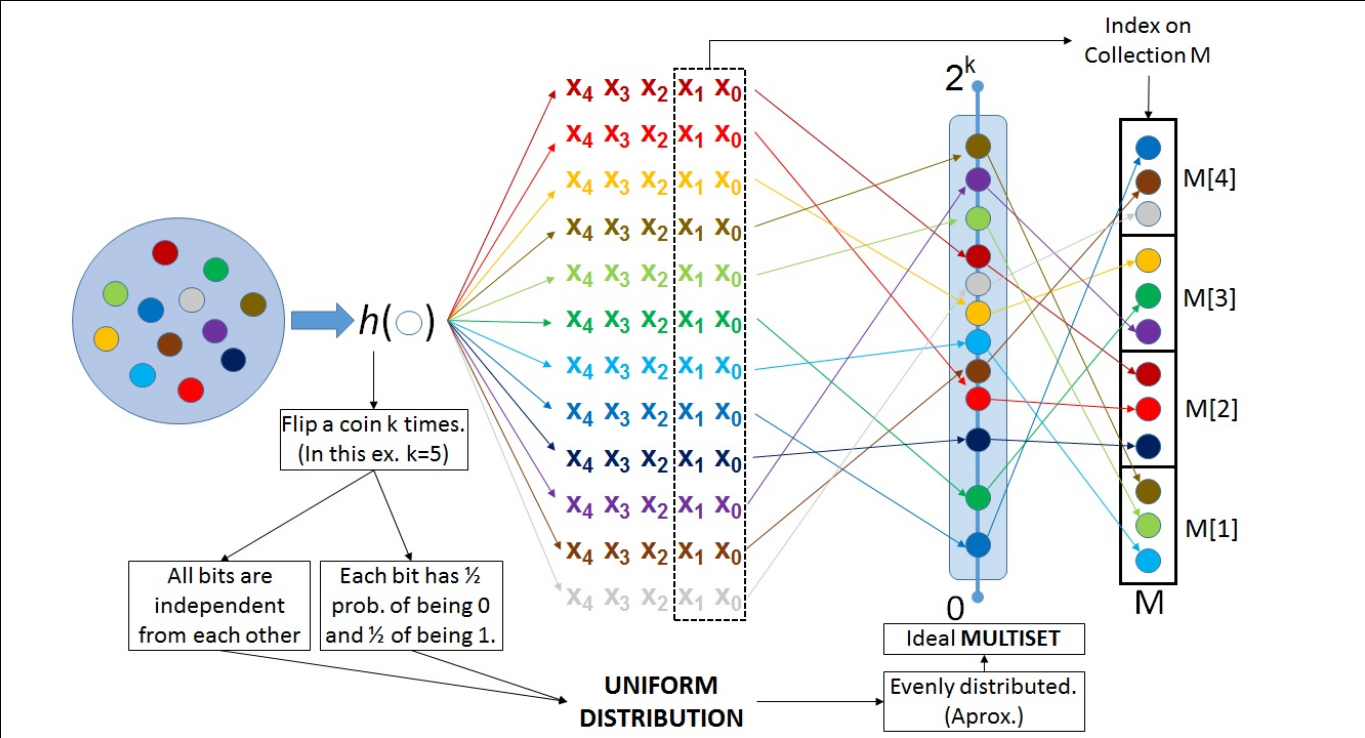
\includegraphics[scale=0.2]{HLL.png}
\caption Thuật toán Hyper Log Log
\end{figure}
\end{frame}
\begin{frame}
\begin{figure}[H]
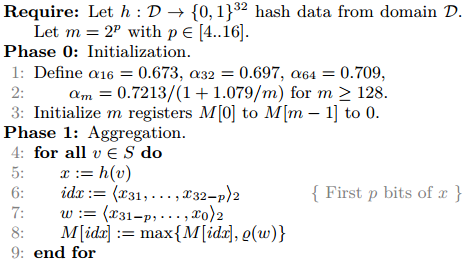
\includegraphics[scale=0.3]{HLL1.png}

\end{figure}
\end{frame}
\begin{frame}
\begin{figure}[H]
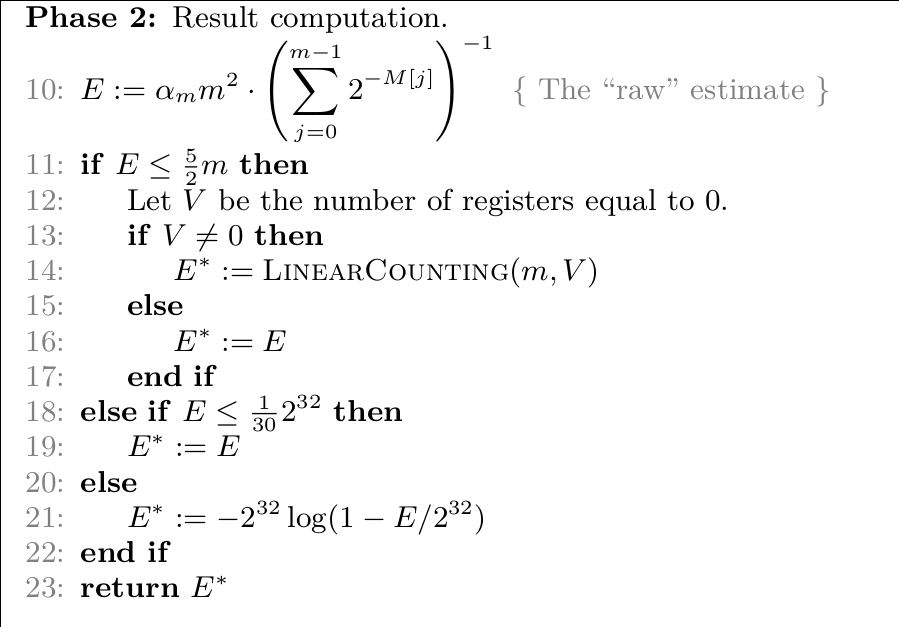
\includegraphics[scale=0.3]{HLL2.png}
\end{figure}
\end{frame}
\begin{frame}{Giải thích chi tiết }
\begin{enumerate}
\item Initialization of registers
\item Small range correction
\item Large range corrections.
\end{enumerate}
\end{frame}
\begin{frame}{Sử dụng hàm băm 64 bit}
\begin{itemize}
\item[•] Hàm băm L bits có thể có $2^L$ giá trị phân biệt. Nếu lực lượng của tập n có $2^L$ biểu diễn thì xung đột hàm băm có khả năng nhiều xảy ra $\rightarrow$ ước lượng chính xác là không thể.
\item[•] Yêu cầu bộ nhớ $\lceil log_2(L + 1 - p) \rceil .2^p$ bits
\begin{itemize}
\item L bits hàm băm, độ chính xác p.
\end{itemize}
\item[•] Sử dụng 64 bits yêu cầu bộ nhớ $6.2^p$
\begin{itemize}
\item không cần quan tâm xung đột hàm băm (lực lượng tập $2^64 \approx 1.8\cdot 10^{19}$ )
\item Large range correction là không cần thiết 
\end{itemize}
\end{itemize}
\end{frame}
\section*{Tài liệu tham khảo}

% TODO: Book
\begin{frame}{Sách tham khảo}
    \vspace{20pt}

    \bi
        \item {\color{hilight}Competitive Programming} by Steven Halim
        \item[] (Sử dụng bản 2 hoặc bản 3)
        \vspace{10pt}
        \item {\color{hilight}Bài giảng Chuyên đề} by Lê Minh Hoàng
    \ei
\end{frame}

% TODO: Overview
\begin{frame}{Các bài giảng}
 
\end{frame}

% TODO: What kind of problems we're dealing with: description/input/output



\end{document}
